\subsection{One-Dimensional Unconstrained Optimization - Chapter 13}

Often times it is important to find the most efficient or cost
effective solution to a particular design. The Newton-Raphson method
depicted below is a widely used method for optimization. Note however
that any search method can be adapted for use in optimization. 

\begin{enumerate}

\item {\bf Classical Optimization}

Classically optimization is written in the form like the equation
below

\begin{equation}
find~x~such~that~min(f(x))
\end{equation}

A very simple example is where $f(x) = x^2-1$. The solution to this
equation can be solved by computing where the derivative $\partial
f/\partial y = 2x = 0$. In this case the function is a minimum when
$x=0$ and the minimum value is negative -1. Care must be taken however
when using this method because finding where the partial derivative is
zero is actually finding a local extrema. For example, if $f(x) = -x^2
+ 8x -12$, the first derivative is zero when $x = 4$ which yields
$f(4) = 4$ however simple inspection shows that when $x=0$, $f(0)=-12$
which is smaller than 4. This is because the method above has found a
maximum instead of a minimum. Suppose however that you cannot solve
the first derivative? For example, try and solve for the minimum
below

\begin{equation}
f(x) = 5(2+\frac{3}{x^4})x^2
\end{equation}

For problems such as this it is sometimes easier to employ a numerical
method. The most widely popular method is the Newton-Raphson method.

\item{\bf Newton-Raphson}

The goal of an optimization problem is similar to a root finding
problem. The difference is that instead of finding where $f(x)=0$
optimization problems seek to find where $f'(x)=0$. Thus the
Newton-Raphson technique can be easily modified to write

\begin{equation}
x_{i+1} = x_i - \frac{f'(x_i)}{f''(x_i)}
\end{equation}

If the relationship $g(x)=f'(x)$ is defined then the equation becomes

\begin{equation}
x_{i+1} = x_i - \frac{g(x_i)}{g'(x_i)}
\end{equation}

which is exactly the same equation as the original Newton-Raphson
technique using $g(x)$ instead of $f(x)$. The issue is that if the
first derivative does not exist, it means the second derivative also
does not exist. Thus, the two derivatives must both be determined
numerically in order to use Newton-Raphson for optimization
problems. Typically the second spatial derivative is replaced such
that

\beq
f''(x_i) =  \frac{f(x_{i+1}) - 2f(x_{i}) + f(x_{i-1})}{\Delta x^2}
\eeq

and 

\beq
f'(x_i) = \frac{f(x_{i+1}) - f(x_{i-1})}{\Delta x}
\eeq

The method above is called the secant method.

\item{\bf Convergence Criteria}

Optimization methods are iterative methods just like everything else
in numerical methods. The stop criterion is setup such that
convergence is reached when $\epsilon_a \le \epsilon_s$ where $\epsilon_s$ is a
user defined parameter whereas $\epsilon_a$ is equal to the equation
below.

\beq
\epsilon_a = \frac{current\_estimate - last\_estimate}{current\_estimate}
\eeq

\item {\bf Gradient Search}

Often times computing the second derivative for the Newton-Raphson
technique is difficult. Another method which is very similar is the
gradient or steepest descent method. 

\beq
x_{n+1} = x_{n} - \alpha \nabla f(x_n)
\eeq

where $\alpha$ is a number between 0 and 1 which is used to slow down
the descent search to ensure the iteration steps to not diverge. 

\item {\bf Parabolic Interpolation}

Although, least squares regression is not covered until section
\ref{s:lsr}, it is possible to obtain a close form expression for a
parabola that approximates the equation trying to be optimized. To do
this, three coordinates ($x_0,x_1,x_2$) are taken that straddle the assumed
optimum. The equation below is then used iteratively until the system
converges. 

\beq
x_3 =
\frac{f(x_0)(x_1^2-x_2^2)+f(x_1)(x_2^2-x_0^2)+f(x_2)(x_0^2-x_1^2)}{2f(x_0)(x_1-x_2)+2f(x_1)(x_2-x_0)+2f(x_2)(x_0-x_1)}
\eeq

\item {\bf Adaptation of Bi-Section - Grid Search}

  Notice however that when using the Newton-Raphson method, the
  second derivative of the function must be known. It is possible to
  use the secant method and numerically obtain the second derivative
  however if the system is well behaved, a simple grid search can be
  used to solve the problem. 

  The bi-section method can be adapted to perform optimization by
  changing the switch criteria from this
  \ \\

  {\it Change the sign of $\Delta x_{n+1}$, if $sign(f(x_n)) \sim=
    sign(f(x_{n+1}))$}
  \ \\

  to this
  \ \\ 

  {\it Change the sign of $\Delta x_{n+1}$, if $f(x_{n+1}) \le
    f(x_{n})$}

  The algorithm basically amounts to keep stepping forward until your
  function becomes smaller. Once it does switch the sign and halve the
  distance until the step size is smaller than an exit criteria.

\item {\bf Ladder Problem}

  Assume a ladder is to be used to paint a wall. Unfortunately there
  is a fence a distance $d$ from the wall with a height of $h$. Solve
  for the minimum distance $L$ of the ladder. {\bf Draw a picture to
    help}. 

  To start solving this problem we define a coordinate system and let
  the ladder be defined by $y = mx+b$ where $b$ is the position of the
  ladder on the wall and $-b/m$ is the x distance from the
  wall. Obviously $m$ will be negative. Since this is a minimization
  problem, the smallest ladder will be touching the fence such that $h
  = md+b$ or rather $b = h - md$

  Using the Pythagorean Theorem, we know that $L^2 = b^2 +
  (b^2/m^2)$. Substituting $b=h-md$ into the equation for length
  yields

  \begin{equation}
    L^2 = (h-md)^2 + (h-md)^2/m^2
  \end{equation}

  Since the height of the fence is known $h=4~m$ and the distance from
  the wall is known $d = 4~m$, the equation above is in the form
  $find~m~to~min(L(m))$. At this point we can use Grid Search,
  Newton-Raphson or Gradient Search to solve this problem.

\end{enumerate}

\subsection {Multi-Dimensional Unconstrained Optimization}

\begin{enumerate}

\item {\bf Analytic Method}

Suppose that we want to minimize

\begin{equation}
p = -8\rho + \rho^2 + 12 T + 4T^2 - 2\rho T
\end{equation}

Analytically we would simply set the gradient equal to zero.

\begin{equation}
  \nabla p = \begin{Bmatrix} \frac{\partial
      p}{\partial \rho}
    \\ \frac{\partial p}{\partial T}\end{Bmatrix} = \begin{Bmatrix} -8
    + 2\rho -2T \\ 12 + 8T - 2\rho \end{Bmatrix} = \vec{0}
\end{equation}

This yields a system of equations which can be solved using Gaussian
substitution or matrix inversion. The solution is $\rho = 3.33$ and $T
= -0.667$. 

\item{\bf Grid Search}

In order to perform grid search in 1 dimensions you simply evaluate
the function one step to the left and to the right. Formally this can
be written as $f(x_0-\Delta x)$ and $f(x_0+\Delta x)$. However in two
dimensions, the number of function evaluations becomes 8. That is,
$f(x_0+\Delta x,y_0)$, $f(x_0-\Delta x,y_0)$, $f(x_0,y_0+\Delta y)$,
$f(x_0,y_0-\Delta y)$, $f(x_0-\Delta x,y_0-\Delta y)$, $f(x_0+\Delta
x,y_0-\Delta y)$, $f(x_0-\Delta x,y_0+\Delta y)$, and $f(x_0+\Delta
x,y_0+\Delta y)$. The rules are the same, continue to move towards the
smallest of the 8 and if you cannot reduce the function size anymore,
halve the step size until an exit criteria. This method becomes large
rather quickly. The function evaluations is equal to
$\sum\limits_{i=0}^{D-1} 2^{i+1}(D-i)$ where D
is the order. When $D=1$ the function evaluations is 2D = 2, when
$D=2$ the function evaluations is 2D+4(D-1) = 4+4 = 8, when $D=3$ the
function evaluations is 2D+4(D-1)+8(D-2) = 6+12+8=26, $D=4$ yields
2D+4(D-1)+8(D-2)+16(D-3) = 8+12+16+16 = 52. That's alot of function
evaluations. A simple computer program can be programmed to do this
but the gradient search is alot better.

\item {\bf Gradient Search}

The gradient search in multiple dimension is extremely easy to employ
and often the easiest to code as well.

\beq
\vec{x}_{n+1} = \vec{x}_n - \alpha \nabla f(\vec{x}_n)
\eeq

The simplicity lies in the equations ability to handle multiple
dimensions much easier than other methods such as Grid Search or
Newton-Raphson. 

\end{enumerate}

\subsection { Linear Constrained Optimization - Chapter 15}

All engineering problems have constraints. Time constraints, storage
constraints, load constraints, you name it. It is impossible to make
something too big. At some point there will be diminishing returns and
it will be better to make less of something than more of
something. Most problems are non-linear and require the use of
Lagrange Multipliers but that is beyond the scope of this
course. Thus, only linear constrained optimization problems will be
considered in this course. 

\begin{enumerate}

\item {\bf Gas-Processing Plant}

  Suppose a gas-processing plant receives a fixed amount of raw gas
  each week. Gas is processed into two grades regular and
  premium. Only 1 type of gas can be processed at one time. The
  facility is open 80 hrs/week using two shifts and receives 77 $m^3$
  of raw gas per week. The regular gas requires 7 $m^3$ of raw gas per
  tonne and the premium gas requires 11 $m^3$ of raw gas per
  tonne. The regular gas requires 10 hrs to produce 1 tonne while the
  premium gas requires 8 hrs to produce 1 tone. The plant has storage
  constraints and can only store 9 tonnes of regular gas and 6 tonnes
  of premium gas. Assume the company sells all the regular gas
  produced at the end of the week at \$150/tonne and the premium gas
  at \$175 per tonne. How much regular and premium gas should be made
  to maximize profit.

  If $x_1$ = amount of regular gas and $x_2$ is the amount of premium
  gas the problem can be set up using the equations to the left. In
  order to solve this problem using a Mathematics toolbox however
  requires problem to be cast into the form shown on the right where
  the profit function has been inverted, becomes a minimization
  problem and the inequalities are cast in the form of $g(x) \le 0$

  $$ 
  \begin{array}{llcll}
    \mbox{Maximize}  &f(x_1,x_2) = 150\,x_1 + 175\,x_2 ~~~~~
    &&\mbox{Minimize} &f(x_1,x_2) = -(150\,x_1 + 175\,x_2) \\
    \mbox{subject to} &7\,x_1 + 11\,x_2 \le 77 &\Rightarrow ~
    &\mbox{subject to} &7\,x_1 + 11\,x_2 - 77 \le 0 \\
    & 10\,x_1 + 8\,x_2 \le 80 &&& 10\,x_1 + 8\,x_2 -80 \le 0 \\
    & x_1 \le 9  &&& x_1 - 9 \le 0 \\
    & x_2 \le 6  &&& x_2 - 6 \le 0 \\
    & x_1 \ge 0  &&& -x_1 \le 0 \\
    & x_2 \ge 0  &&& -x_2 \le 0
  \end{array}
  $$

  \item {\bf MATLAB Solution}

  Using the form on the right, the equation can be solved using the
  function $fmincon$. Unfortunately, this function is not included in
  Octave (at least at the time this text was written in 2015). In
  order to solve this problem by hand, skip to the next section.

  \begin{framed}
   \begin{verbatim}
     function Ex15_1

     x0 = [1,1];
     options = optimset('LargeScale','off');
     [x,fmin] = fmincon(@objfun,x0,[],[],[],[],[],[],@confun,options);
     x_o = x
     fmax =-fmin

     function f = objfun(x)
     f = -(150*x(1) + 175*x(2));  
     
     function [c,ceq] = confun(x)
     c = [7*x(1) + 11*x(2) - 77;
       10*x(1) + 8*x(2) - 80;
       x(1) - 9;
       x(2) - 6;
       -x(1);
       -x(2)];
     ceq = [];  
   \end{verbatim}
  \end{framed}

  In the function above the first function Ex15\_1 sets up the
  problem. objfun is the objective function to be solved and confon is
  the constraints where c contains the inequality constraints and ceq
  contains the equality constraints. 

\item {\bf Graphical Solution}

  In order to solve linear programming problems, the constraints must
  first be graphed. 

  \begin{figure}[H]
    \begin{center}
      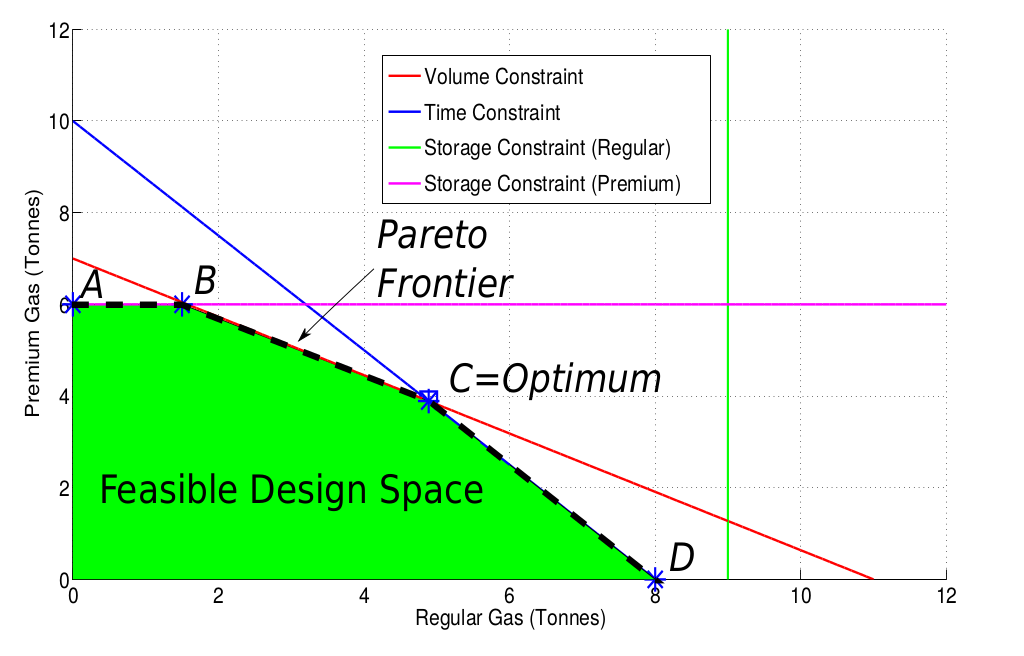
\includegraphics[height=0.45\textwidth,width=0.75\textwidth]{Graphics/Gas_Processing}
    \end{center}
  \end{figure}

  The graph has a lot of information on it so let's walk through this
  graph slowly. The x-axis is the amount of regular gas in tonnes and
  the y-axis is the amount of premium gas in tonnes. The green and
  magenta lines indicate storage constraints since the plant can only
  store 9 tonnes of regular gas and 6 tonnes of premium gas. The blue
  line shows the time constraint. Since the plant is only open 80
  hrs/week and only 1 gas can be made at a time, the blue line
  indicates the limits on this shortcoming of the factory. The red
  line is similar only it indicates the volume constraint since the
  plant only receives 77 $m^3$ of raw gas per week. The green line is
  a redundant constraint in that if it is removed, the problem stays
  the same; however, the other 3 lines create the feasible design
  space as indicated by the large green space. The intersection of
  each of the constraints lines with each other and the x and y-axes
  are critical design points which designate the Pareto Frontier. The
  optimum design choice is one of these 4 points. Each point can be
  solved for explicitly using Gaussian subsitution and plugging each
  coordinate into the profit function. Inspection shows that point C
  is the optimum design choice. $x_1 = 4.89$, $x_2 = 3.89$ and
  $Profit = \$1413.89$. 

\end{enumerate}

